\documentclass[12pt]{article}\usepackage[]{graphicx}\usepackage[]{xcolor}
% maxwidth is the original width if it is less than linewidth
% otherwise use linewidth (to make sure the graphics do not exceed the margin)
\makeatletter
\def\maxwidth{ %
  \ifdim\Gin@nat@width>\linewidth
    \linewidth
  \else
    \Gin@nat@width
  \fi
}
\makeatother

\definecolor{fgcolor}{rgb}{0.345, 0.345, 0.345}
\newcommand{\hlnum}[1]{\textcolor[rgb]{0.686,0.059,0.569}{#1}}%
\newcommand{\hlsng}[1]{\textcolor[rgb]{0.192,0.494,0.8}{#1}}%
\newcommand{\hlcom}[1]{\textcolor[rgb]{0.678,0.584,0.686}{\textit{#1}}}%
\newcommand{\hlopt}[1]{\textcolor[rgb]{0,0,0}{#1}}%
\newcommand{\hldef}[1]{\textcolor[rgb]{0.345,0.345,0.345}{#1}}%
\newcommand{\hlkwa}[1]{\textcolor[rgb]{0.161,0.373,0.58}{\textbf{#1}}}%
\newcommand{\hlkwb}[1]{\textcolor[rgb]{0.69,0.353,0.396}{#1}}%
\newcommand{\hlkwc}[1]{\textcolor[rgb]{0.333,0.667,0.333}{#1}}%
\newcommand{\hlkwd}[1]{\textcolor[rgb]{0.737,0.353,0.396}{\textbf{#1}}}%
\let\hlipl\hlkwb

\usepackage{framed}
\makeatletter
\newenvironment{kframe}{%
 \def\at@end@of@kframe{}%
 \ifinner\ifhmode%
  \def\at@end@of@kframe{\end{minipage}}%
  \begin{minipage}{\columnwidth}%
 \fi\fi%
 \def\FrameCommand##1{\hskip\@totalleftmargin \hskip-\fboxsep
 \colorbox{shadecolor}{##1}\hskip-\fboxsep
     % There is no \\@totalrightmargin, so:
     \hskip-\linewidth \hskip-\@totalleftmargin \hskip\columnwidth}%
 \MakeFramed {\advance\hsize-\width
   \@totalleftmargin\z@ \linewidth\hsize
   \@setminipage}}%
 {\par\unskip\endMakeFramed%
 \at@end@of@kframe}
\makeatother

\definecolor{shadecolor}{rgb}{.97, .97, .97}
\definecolor{messagecolor}{rgb}{0, 0, 0}
\definecolor{warningcolor}{rgb}{1, 0, 1}
\definecolor{errorcolor}{rgb}{1, 0, 0}
\newenvironment{knitrout}{}{} % an empty environment to be redefined in TeX

\usepackage{alltt}

%\usepackage[roman]{../pres1}
%\usepackage[sans]{../pres1}

\usepackage[hmargin=1in,vmargin=1in]{geometry}
\usepackage{parskip}
\usepackage{hyperref}
\usepackage{graphicx}
\hypersetup{pdfstartview=FitV,hidelinks}



\IfFileExists{upquote.sty}{\usepackage{upquote}}{}
\begin{document}

{
  \Large
  \centering
  Lab 6 Assignment --- Models of Interspecific Interactions \\
  Due by 8:00am on Monday \par
}

Answer each of the following questions and upload your Excel file and
R script to ELC. Be sure to show your calculations. Undergraduates
only have to do Exercise I in R.  \\


\vspace{6pt}

{\bf Exercise I \\}
You are studying the dynamics of jaguar (\textit{Panthera onca}) and Baird's
tapir (\textit{Tapirus bairdii}) in Costa Rica's Corcavodo National Park. After
years of research, you obtain the following parameter estimates, which
you would like to use in a Lotka-Volterra model: $r^{prey}=0.05$,
$k^{pred}=0.0005$, $b^{pred}=0.001$, and $d^{pred}=0.45$.  
\begin{enumerate}
  \item[(A)] What predator population size corresponds to prey equilibrium?
    What prey population size corresponds to predator equilibrium? 
  \item[(B)] Project the populations 100 years following an initial prey
    population size of $N_0^{prey}=500$ and an initial predator
    population size of $N_0^{pred}=100$. Plot the projections.  
  \item[(C)] Clearly, these populations have not reached a stable
    equilibrium, so what is the interpretation of the equilibrium
    values from part (a)? What happens if you set the initial
    population sizes to the equilibrium values?  
  %% \item[(D)] Change the value of $r^{prey}$ from 0.05 to 0.1,
  %%   and recalculate the equilibrium points for prey and
  %%   predators. Project the dynamics of both species again. Plot the
  %%   results. What are the primary differences?  What explains these
  %%   differences? 
\end{enumerate}

\vspace{12pt}

\begin{figure}[h!]
  \centering
  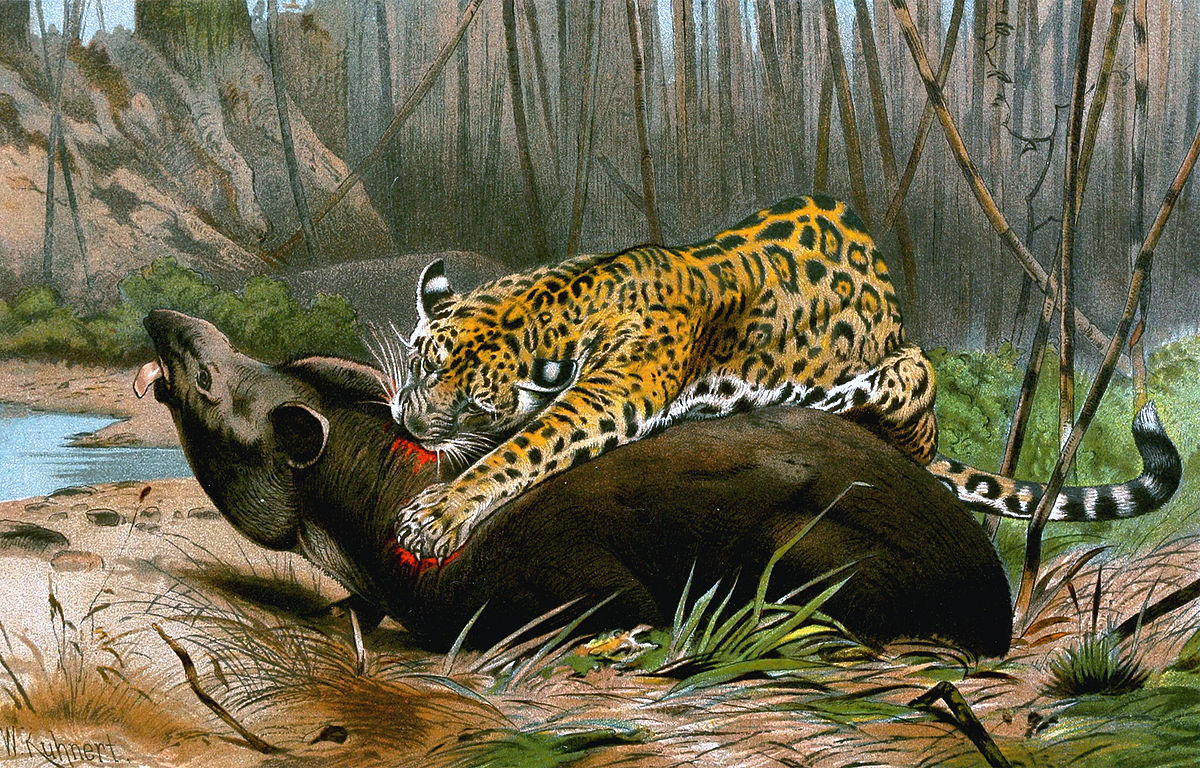
\includegraphics[width=0.85\textwidth]{jaguar_killing_tapir}
%  \caption{Jaguar and tapir}
  \label{fig:jag-tapir}
\end{figure}


\clearpage

{\bf Exercise II \\}
The Canada warbler (\textit{Cardellina canadensis}) and the hooded
warbler ({\it Stetophaga citrina}) are two species of
Neotropical-Nearctic migratory birds that appear to compete for the
same resources where their ranges meet in the southern Appalachian
Mountains. Assume their dynamics follow the Lotka-Volterra competition
model with parameters $r^{A}=0.2$, $r^{B}=0.3$,
$K^{A}=250$, $K^{B}=200$, $\alpha^{A}=0.1$, and 
$\alpha^{B}=0.1$.   
\begin{enumerate}
  \item[(A)] Plot 25 years of dynamics following initial conditions of 
    $N_0^A = 200$ and $N_0^B=50$.  
  \item[(B)] What are the 2 equilibrium values for these species?
  \item[(C)] Do these conditions describe stable coexistence,
    competitive exclusion, or unstable equilibrium?  
  \item[(D)] What is the minimum value of $\alpha^B$ that would result in
    competitive exclusion of species A? (Hint: Use the equilibrium
    equations to solve for $\alpha^B$). Plot 25 years of dynamics under
    this scenario. Use the same initial abundance values as before. 
\end{enumerate}


\vspace{12pt}

\begin{figure}[h!]
  \centering
  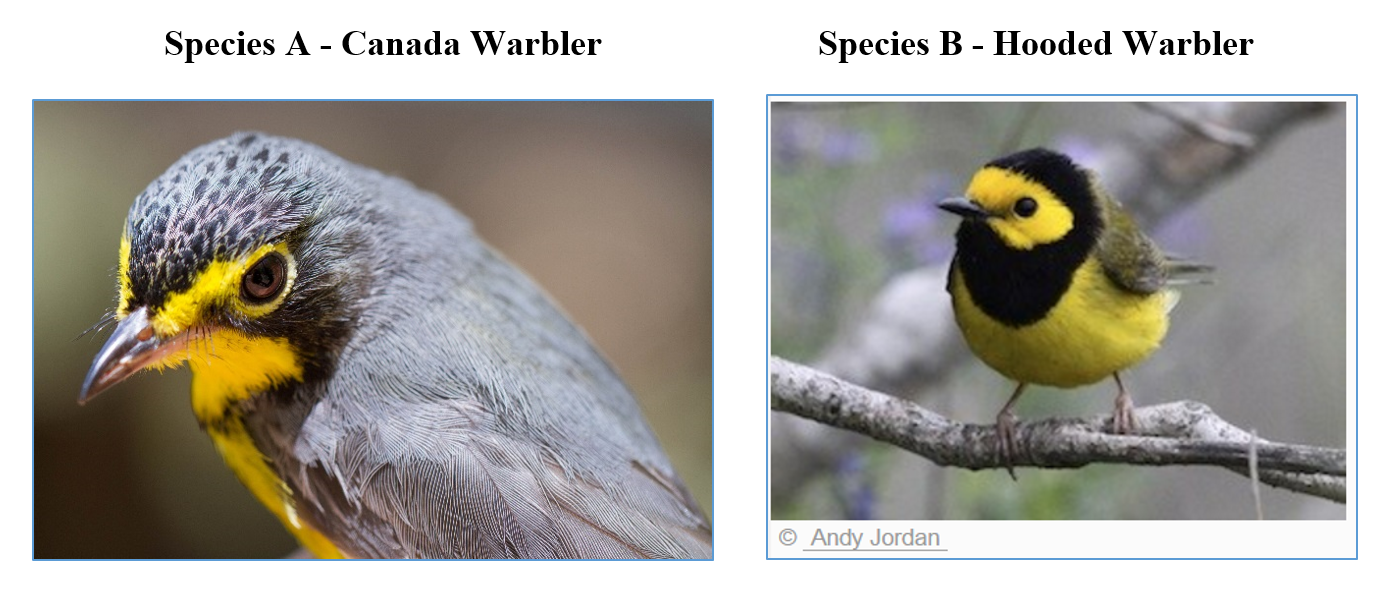
\includegraphics[width=\textwidth]{cawa-howa}
  \label{fig:cawa-howa}
\end{figure}


\clearpage

{\bf R example \\}


\begin{knitrout}
\definecolor{shadecolor}{rgb}{0.969, 0.969, 0.969}\color{fgcolor}\begin{kframe}
\begin{alltt}
\hldef{nYears} \hlkwb{<-} \hlnum{5000}
\hldef{r.prey} \hlkwb{<-} \hlnum{0.01}
\hldef{k.pred} \hlkwb{<-} \hlnum{0.00001}
\hldef{b.pred} \hlkwb{<-} \hlnum{0.00001}
\hldef{d.pred} \hlkwb{<-} \hlnum{0.01}
\hldef{N.prey} \hlkwb{<-} \hlkwd{rep}\hldef{(}\hlnum{NA}\hldef{, nYears)}
\hldef{N.pred} \hlkwb{<-} \hlkwd{rep}\hldef{(}\hlnum{NA}\hldef{, nYears)}
\hldef{N.prey[}\hlnum{1}\hldef{]} \hlkwb{<-} \hlnum{1000}
\hldef{N.pred[}\hlnum{1}\hldef{]} \hlkwb{<-} \hlnum{300}
\hlkwa{for}\hldef{(t} \hlkwa{in} \hlnum{2}\hlopt{:}\hldef{nYears) \{}
    \hldef{N.prey[t]} \hlkwb{<-} \hldef{N.prey[t}\hlopt{-}\hlnum{1}\hldef{]} \hlopt{+} \hldef{N.prey[t}\hlopt{-}\hlnum{1}\hldef{]}\hlopt{*}\hldef{(r.prey}\hlopt{-}\hldef{k.pred}\hlopt{*}\hldef{N.pred[t}\hlopt{-}\hlnum{1}\hldef{])}
    \hldef{N.pred[t]} \hlkwb{<-} \hldef{N.pred[t}\hlopt{-}\hlnum{1}\hldef{]} \hlopt{+} \hldef{N.pred[t}\hlopt{-}\hlnum{1}\hldef{]}\hlopt{*}\hldef{(b.pred}\hlopt{*}\hldef{N.prey[t}\hlopt{-}\hlnum{1}\hldef{]} \hlopt{-} \hldef{d.pred)}
\hldef{\}}
\hlkwd{plot}\hldef{(}\hlnum{1}\hlopt{:}\hldef{nYears, N.prey,} \hlkwc{type}\hldef{=}\hlsng{"l"}\hldef{,} \hlkwc{col}\hldef{=}\hlsng{"black"}\hldef{,} \hlkwc{ylim}\hldef{=}\hlkwd{c}\hldef{(}\hlnum{0}\hldef{,} \hlnum{3500}\hldef{),}
     \hlkwc{xlab}\hldef{=}\hlsng{"Year"}\hldef{,} \hlkwc{ylab}\hldef{=}\hlsng{"Abundance"}\hldef{)}
\hlkwd{lines}\hldef{(}\hlnum{1}\hlopt{:}\hldef{nYears, N.pred,} \hlkwc{type}\hldef{=}\hlsng{"l"}\hldef{,} \hlkwc{col}\hldef{=}\hlsng{"blue"}\hldef{)}
\hlkwd{legend}\hldef{(}\hlnum{1}\hldef{,} \hlnum{3500}\hldef{,} \hlkwd{c}\hldef{(}\hlsng{"Prey"}\hldef{,} \hlsng{"Predator"}\hldef{),} \hlkwc{lty}\hldef{=}\hlnum{1}\hldef{,} \hlkwc{col}\hldef{=}\hlkwd{c}\hldef{(}\hlsng{"black"}\hldef{,} \hlsng{"blue"}\hldef{))}
\end{alltt}
\end{kframe}

{\centering \includegraphics[width=0.75\textwidth]{figure/pred-prey-1} 

}


\end{knitrout}



\end{document}

